\begin{frame}{The algorithms in C++}
	\begin{center}
		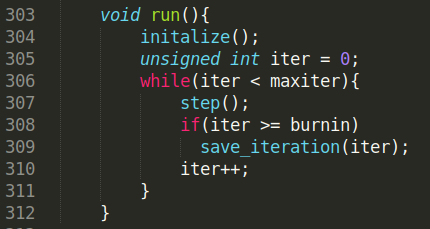
\includegraphics[scale=0.4]{../etc/neal8_2.png}
	\end{center}
	\begin{itemize}
		\item Example: Normal-NormalInvGamma hierarchy, no hyperpriors
		\item \texttt{initalize()}: random allocation
		\item \texttt{step()}
		\begin{itemize}
			\item \texttt{sample\_allocations()}: vector \texttt{card} of cardinalities of clusters
			\item 4 cases handled separately: singleton vs !singleton, aux vs old
			\item \texttt{sample\_unique\_values()}: vector \texttt{clust\_idxs} to record which data are in each cluster
		\end{itemize}
		\item Actual cluster structures?
	\end{itemize}
\end{frame}


\begin{frame}{Impending extensions}
	\begin{itemize}
	   \item \textbf{Hyperpriors}: objects of class \texttt{Hypers} store pointers to objects of class \texttt{HypersFixed} %TODO?
	   \item \textbf{Non-conjugacy}: via Stan's HMC sampler
	   \item  \textbf{R interface}: via \textbf{protocol buffers}
	\end{itemize}
\end{frame}

\begin{frame}{Protocol Buffers}
	\begin{itemize}
		\item API developed by Google
		\item Data is saved in XML-like structures, called \textbf{messages}, that are defined in \texttt{.proto} files
		\item Each message corrresponds to a class in C++
		\item The \texttt{protoc} compiler produces the C++ files that make up the API
		\item RProtoBuf
		\item Compromise between efficiency and human-readibility
	\end{itemize}
\end{frame}

\begin{frame}{A general library?}
	%è possibile una libreria del tutto "generale"? Utilizzando una libreria tipo stan per le distribuzioni, si può mettere su un codice per cui non serve programmare a mano gli update dei valori dei cluster e dei vari iper-parametri, volendo rinunciare a degli update coniugati? %TODO what
\end{frame}


